\section{Анализ языковых моделей}

В результате обучения моделей и тестирования различных архитектур, были получены результаты для семи различных моделей. Исходные данные для обучения и валидации были одни и теже --- текстовый корпус, разделенный две выборки, обучающую и валидационную, 0.85 и 0.15 от всего датасета соответственно. Итоговое значение perplexity измерялось именно на валидационной выборке.

\subsection{Kneser-Nay}

Для модели Kneser-Nay проводилось два эксперимента: при использовании три-граммной и пятиграммной вариаций. Различия данных моделей заключаются в количестве символов, которые учитываются при предсказании. Использование более 5 токенов становится затратно по памяти, поэтому эксперименты для больших значений не проводились. Так как Kneser-Nay --- это статистическая модель, у нее нет как такового цикла обучения. Предобработка заключается в подсчете всех необходимых n-грамм, которые используются при вычислении вероятностей на этапе генерации. Поэтому метрики train loss и val loss для данных моделей отсутствуют.

По результатам экспериментов, 5-граммная модель ожидаемо показала себя лучше. Время на создание моделей затрачено в пределах одного часа, при этом достаточно использования только обычных процессоров --- графические ускорители излишни, что значительно упрощает и удешевляет создание моделей.

Итоговые значения perplexity составили:

\begin{itemize}
	\item для 3-граммной модели: 67.43;
	\item для 5-граммной модели: 59.92.
\end{itemize}

Основная цель реализации n-граммных моделей было получение бейзлайна. Нейронные сети должны показывать себя лучше статистических моделей, так как они могут запоминать более длинные зависимости, однако чтобы более точно оценивать их эффективность, нужна нижняя граница, которую необходимо превзойти. В качестве такой нижней оценки и выступила архитектура Kneser-nay.

\subsection{LSTM}

Подавляющая часть экспериментов проводилась для архитектуры LSTM. От нее ожидалось наилучшее качество, если не использовать предобученные модели трансформеров. Для имеющегося объема данных рекуррентные сети являются оптимальным решением при решении задачи языкового моделирования.

Для моделей LSTM необходимо было:

\begin{enumerate}
	\item Найти оптимальное количество рекуррентных слоев модели.
	\item Подобрать наилучшие размеры векторных представлений и скрытого состояния слоя LSTM.
	\item Исследовать влияние значения learning rate и косинусного шедулера на скорость сходимости и итоговое качество.
\end{enumerate}

Все эксперименты с LSTM проводились с использовением графического ускорителя Tesla V100-PCIE-32GB. В среднем, обучение моделей занимало около 12 часов, однако для самой большой архитектуры понадобилось примерно в два раза больше времени. Осуществлялись попытки ускорить обучение, увеличив размер батча. Проводились эксперименты с batch\_size 256, 512 и 1024, однако слишком большой размер батча негативно сказывался на итоговом качестве. Поэтому в качестве оптимального значения был выбран $batch\_size = 512$. Загруженность памяти GPU составила порядка 35-40\% (для батча 1024 --- до 95\%). Обучение всех моделей проходило в течение десяти эпох. Train loss логировался каждые 50 итераций, а val loss --- когда проходила десятая часть эпохи.

Базовый эксперимент был проведен для архитектуры LSTM с четырьмя рекуррентными ячейками, размером эмбеддингов 128 и размером скрытого состояния также 128. Графики тренировки представлены на рисунках \ref{fig:lstm_4_128_128_train} и \ref{fig:lstm_4_128_128_val}. На них можно увидеть, что значение функции потерь на валидации довольно быстро сходится к значению 3.6, и дальше процесс оптимизации сильно замедляется. По графику \ref{fig:lstm_4_128_128_train} можно сделать вывод, что следует выбрать архитектуру значительно больше, так как рассмотренная модель не способна достаточно хорошо запомнить имеющийся объем данных. Также было сделано предположение, что использование шедулера также полодительно скажется на качестве, так как постоянное значение learning\_rate (0.005 в данном эксперименте) может не позволять модели оптимизироваться после нескольких эпох, где оптимальнее более низкий lr.

\begin{figure}[ht]
	\centering
	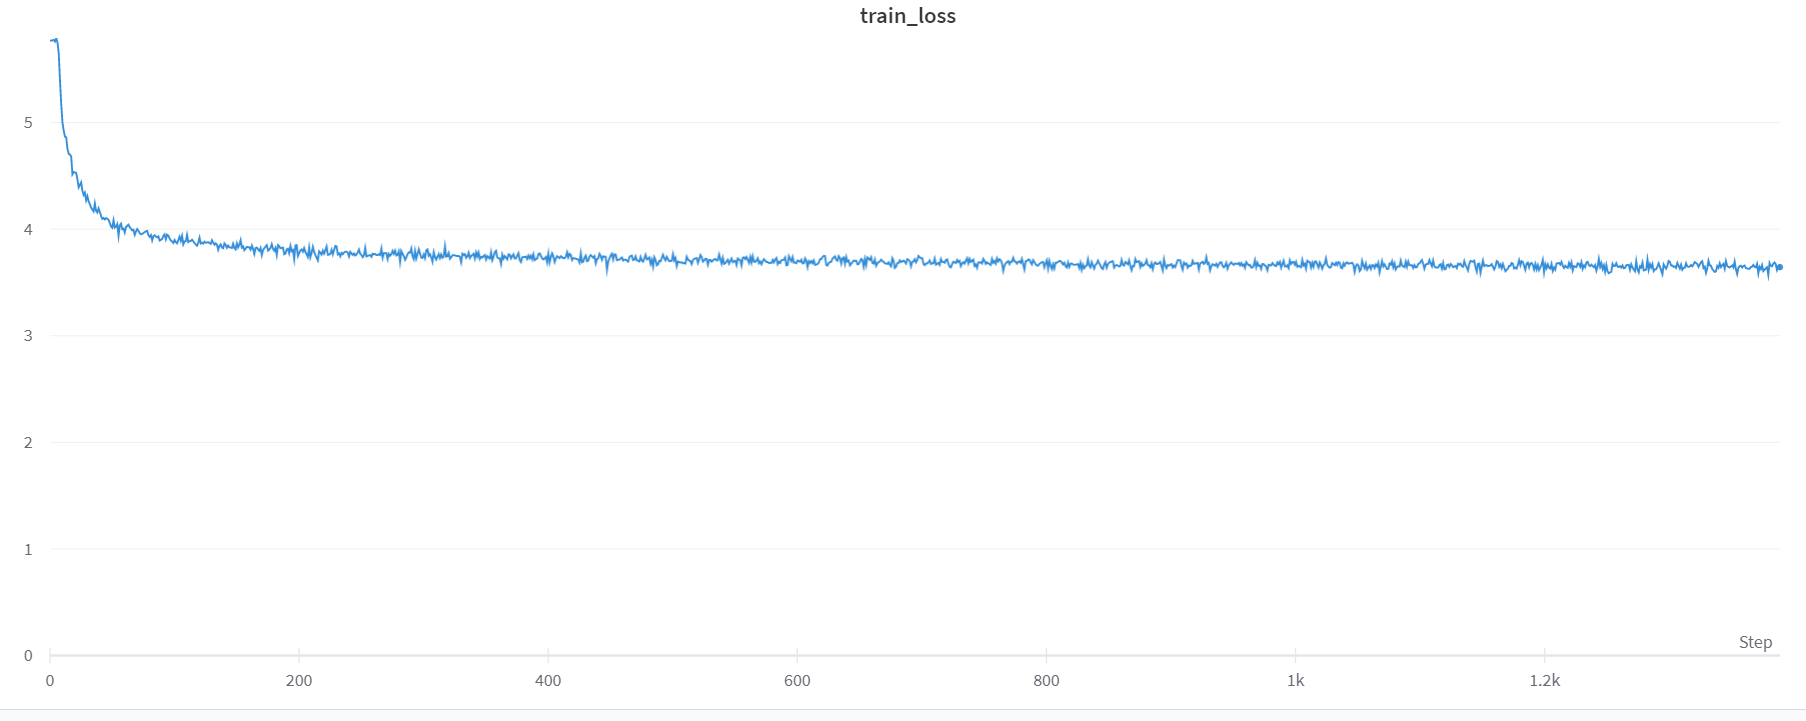
\includegraphics[width=\linewidth]{lstm_avid_train_loss}  
	\caption{ Train loss для LSTM-4-128-128 }
	\label{fig:lstm_4_128_128_train}
\end{figure}

\begin{figure}[ht]
	\centering
	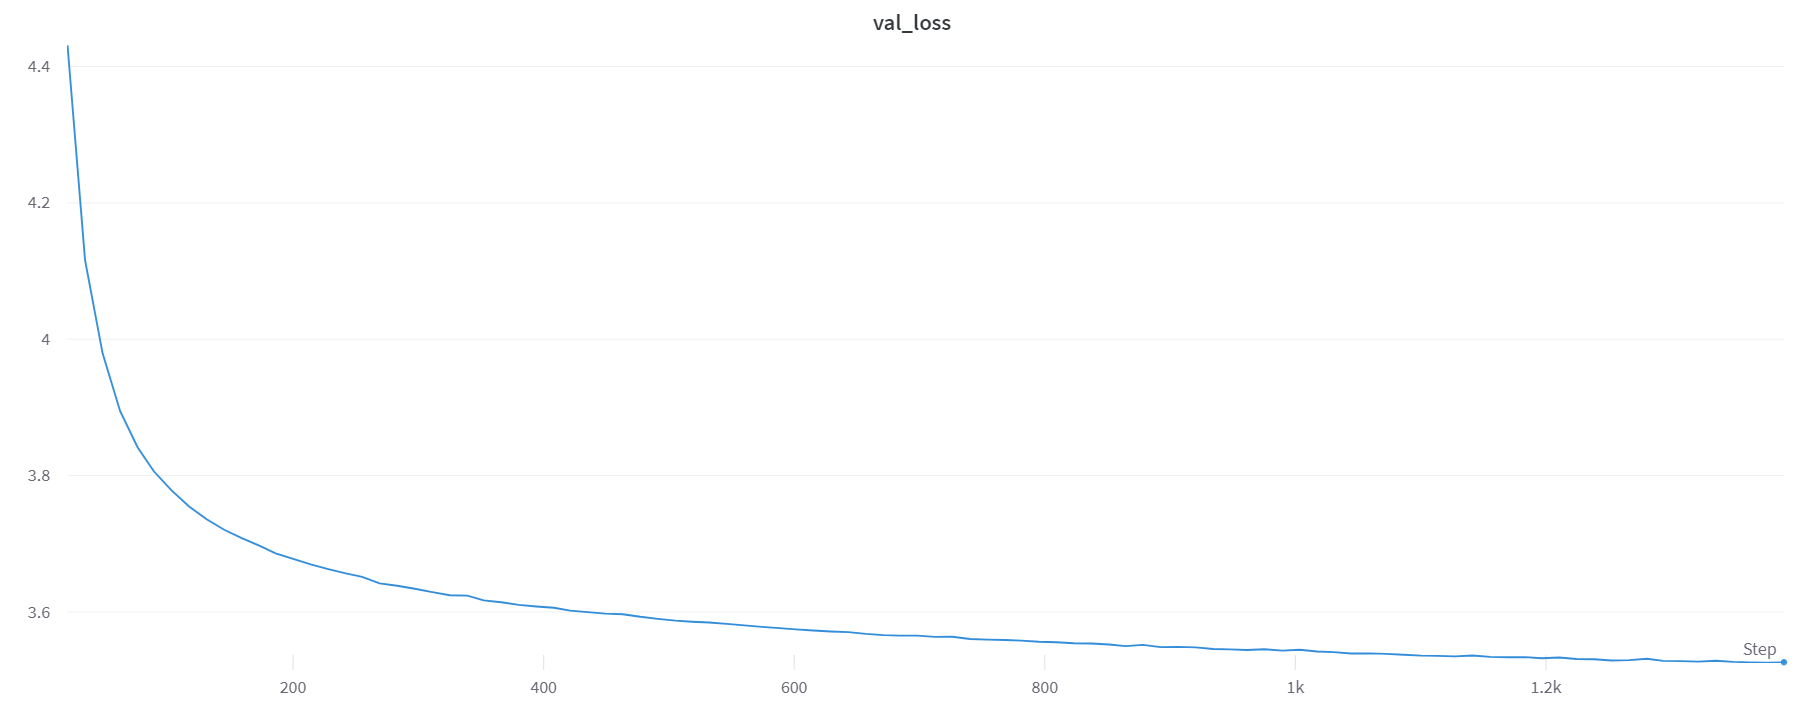
\includegraphics[width=\linewidth]{lstm_avid_val_loss}  
	\caption{ Validation loss для LSTM-4-128-128 }
	\label{fig:lstm_4_128_128_val}
\end{figure}

Следующий эксперимент заключался в увеличении количества параметров модели. Это было достигнуто благодаря увеличению количества рекуррентных ячеек (6 вместо 4), а также увеличения размеров векторных представлений и вектора состояния модели (25 вместо 128). Полученное качество оказалось на 0.1 лучше, чем у предыдущей модели. Однако такое улучшение стоило замедления тренировки почти в 1.5 раза. Графики метрик для тренировки отображены на рисунках \ref{fig:lstm_6_256_256_train} и \ref{fig:lstm_6_256_256_val}.

\begin{figure}[ht]
	\centering
	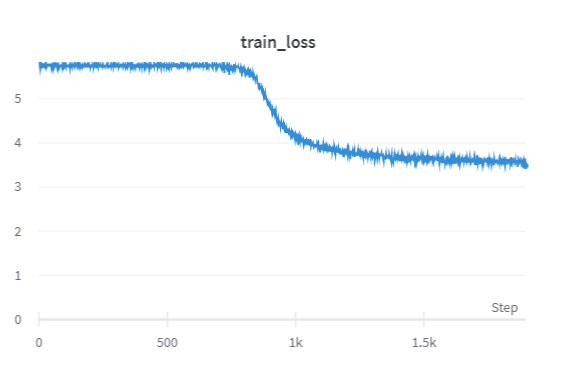
\includegraphics[width=\linewidth]{lstm_grateful_train_loss}  
	\caption{ Train loss для LSTM-6-256-256 }
	\label{fig:lstm_6_256_256_train}
\end{figure}

\begin{figure}[ht]
	\centering
	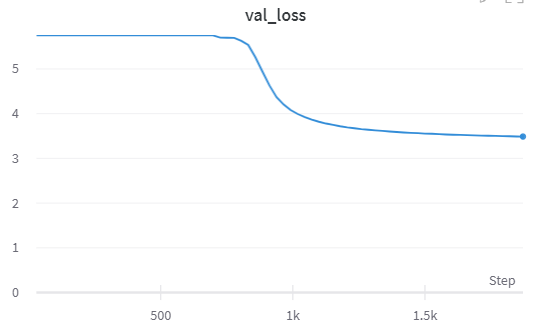
\includegraphics[width=\linewidth]{lstm_grateful_val_loss}  
	\caption{ Validation loss для LSTM-6-256-256 }
	\label{fig:lstm_6_256_256_val}
\end{figure}

По данному эксперименту можно сделать вывод, что архитектура получилась слишком большой. Об этом свидетельствует тот факт, что train loss опускается ниже validation loss, то есть модель начинает переобучаться. В связи с этим, в следующих экспериментах значения embedding\_size и hidden\_size будут меньше.

Следующим шагом была проверка влияния шедулера на процесс обучения. В качестве шедулера применялся косинусный алгоритм, при котором learning rate медленно снижается по косинусоиде. Так как learning rate постепенно снижается, начальное значение выбрано выше, чем в предыдущих экспериментах --- 0,01 вместо 0,005. В качестве размера слоев по результатам предыдущих двух экспериментов выбрано значение 192, количество слоев осталось равно шести. Результаты обучения представлены на рисунках \ref{fig:lstm_6_192_192_train} и \ref{fig:lstm_6_192_192_val}.

\begin{figure}[ht]
	\centering
	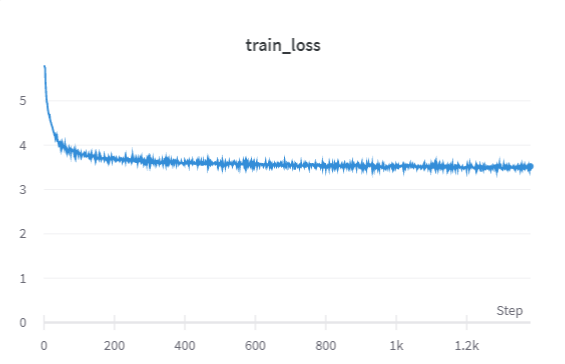
\includegraphics[width=\linewidth]{lstm_laced_train_locc}  
	\caption{ Train loss для LSTM-6-256-256 }
	\label{fig:lstm_6_192_192_train}
\end{figure}

\begin{figure}[ht]
	\centering
	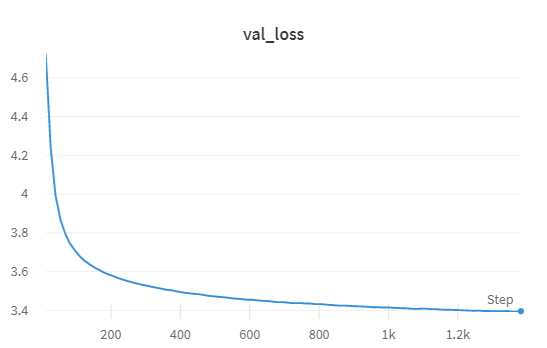
\includegraphics[width=\linewidth]{lstm_laced_val_loss}  
	\caption{ Validation loss для LSTM-6-192-192 }
	\label{fig:lstm_6_192_192_val}
\end{figure}

Данная архитектура с использованием косинусного шедулера показала наилучшее качество с итоговым значением $val\_loss = 3.4$. Можно сделать вывод, что подбор оптимальных размеров слоев, а также оптимизация при помощи шедулера смогли значительно улучшить качество.

В последнем эксперименте осуществлялась попытка увеличить количество слоев в сети LSTM, что могло позволить улучшить качество на длинных последовательностях. Для этого число рекуррентных модулей было увеличено до 8, при этом другие размеры были снижены до 128 для уменьшения общего числа параметров. Кривые обучения можно увидеть на рисунках \ref{fig:lstm_8_128_128_train} и \ref{fig:lstm_8_128_128_val}. Данная модель не смогла выучить никаких зависимостей, итоговое качество наихудшее, даже несмотря на использование косинусного шедулера, аналогично предыдущему эксперименту. Такие результаты можно объяснить тем, что при большом количестве слоев градиенты могут подвергаться затуханию, из-за чего веса модели не оптимизируются.

\begin{figure}[ht]
	\centering
	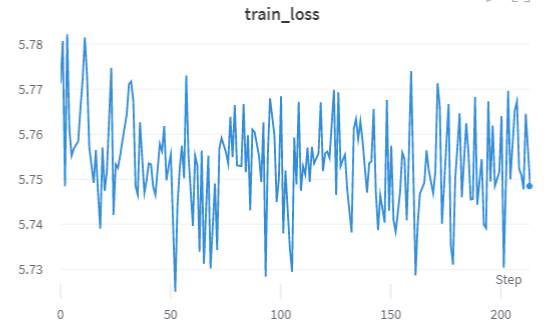
\includegraphics[width=\linewidth]{lstm_vital_train_loss}  
	\caption{ Train loss для LSTM-6-256-256 }
	\label{fig:lstm_8_128_128_train}
\end{figure}

\begin{figure}[ht]
	\centering
	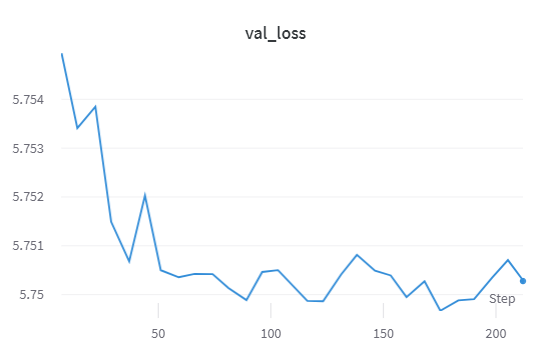
\includegraphics[width=\linewidth]{lstm_vital_val_loss}  
	\caption{ Validation loss для LSTM-8-128-128 }
	\label{fig:lstm_8_128_128_val}
\end{figure}

По архитектуре LSTM на основе проведенных экспериментов можно сделать вывод, что использование косинусного шедулера позволяет ускорить сходимость и улучшить итоговое качество. Также были эмпирически подобраны хорошие параметры рассматриваемой модели, что позволило добиться хорошего качества.

\subsection{GPT-2}

GPT-2 является нейросетевой языковой моделью на основе архитектуры трансформеров, которая в течение нескольких лет являлась наилучшей языковой моделью на ряде датасетов ~\cite{gpt2}. Однако для ее обучения требуются как минимум десятки гигабайт текстовых данных, которые для белорусского языка найти крайне сложно. Поэтому использовалась ее уменьшенная архитектура, distill gpt-2 из библиотеки transformers от huggingface.

GPT-2 содержит гораздо больше параметров, чем рассмотренные архитектуры с использованием LSTM, даже ее дистиллированная версия. Это накладывает ряд ограничений, связанных с размером батча и временем обучения. Такая модель учится в течение нескольких дней, что в том числе связано с архитектурой трансформеров, которая работает за квадратичное время. В результате получена модель, для которой значение perplexity составило 46,14. это можно сравнить с результатами для gpt, полученными на английских датасетах, которые намного больше по объему. На корпусе WikiText103 полная версия GPT-2 дает perplexity 17.48, а дистиллированная версия --- 37.5, что в целом сравнимо с результатами, полученными для белорусских текстов. Основным направлением для улучшения качества является поиск большего объема данных.

Результаты проведенных экспериментов представлены в таблице \ref{table:experiments:metrics}.

\begin{table}[ht]
	\caption{Сравнение метрик для рассмотренных моделей}
	\label{table:experiments:metrics}
	\centering
	\begin{tabular}{|>{\centering}m{0.4\textwidth}|>{\centering}m{0.2\textwidth}|>{\centering}m{0.2\textwidth}|c|}
		\hline
		Модель & Train loss & Val loss & Perplexity \\
		\hline
		Kneser-Nay 3-gram & -- & -- & 67.43 \\
		\hline
		Kneser-Nay 5-gram & -- & -- & 59.92 \\
		\hline
		LSTM-4-128-128 & 3.64 & 3.53 & 49.28\\
		\hline
		LSTM-6-256-256 & 3.48 & 3.49 & 46.73\\
		\hline
		LSTM-6-192-192 + Cosine scheduler & 3.52 & 3.4 & 43.22 \\
		\hline
		LSTM-6-128-128 + Cosine scheduler & 5.74 & 5.75 & 453.28 \\
		\hline
		distill GPT2 & 3.51 & 3.46 & 46.14 \\
		\hline
	\end{tabular}
\end{table}

\subsection{Генерация текста}

Для генерации последовательностей использовался beam search и модель LSTM, для которой получено наилучшее значение метрики perplexity. Процесс генерации по заданному префиксу состоит из следующих шагов:

\begin{enumerate}
	\item Перевод префикса в целочисленный тензор.
	\item Запуск модели на заданном префиксе, получение распределения вероятностей.
	\item Шаг beam search, перераспределение префиксов результатов.
	\item Для каждого луча запуск алгоритма с обновленным префиксом.
\end{enumerate}

При добавлении рандомизации на первый после символа начала строки токен, можно получать полностью сгенерированные предложения. Некоторые примеры, которые удалось получить:

\begin{itemize}
	\item я хацеў пагаварыць з вамi аб усiм
	\item што можа быць лепш за гэта
	\item вы ніколі больш мяне не ўбачыце
\end{itemize}

Такая нейросеть не является оптимальной для генерации длинных текстов, однако с генерацией коротких осмысленных последовательностей справляется неплохо.
